\documentclass[journal]{IEEEtran}
\usepackage{booktabs}
\usepackage{longtable}
\usepackage{array}
\usepackage{graphicx}

\begin{document}

\title{Supplement: Lineage Tables for the 10{,}240-Byte Generator}

\author{The DOPE Project}

\maketitle
\newcommand{\MedDopeCb}{0.940}
\newcommand{\LoDopeCb}{0.914}
\newcommand{\HiDopeCb}{0.976}
\newcommand{\NDopeCb}{97}
\newcommand{\MedGaussCb}{0.656}
\newcommand{\LoGaussCb}{0.431}
\newcommand{\HiGaussCb}{0.803}
\newcommand{\MedChowCb}{0.586}
\newcommand{\LoChowCb}{0.465}
\newcommand{\HiChowCb}{0.637}
\newcommand{\MedIndCb}{-0.012}
\newcommand{\LoIndCb}{-0.020}
\newcommand{\HiIndCb}{-0.00649}
\newcommand{\HolmGaussCb}{1.35\times 10^{-13}}
\newcommand{\HolmChowCb}{4.85\times 10^{-16}}
\newcommand{\HolmIndCb}{1.17\times 10^{-16}}
\newcommand{\SignHolmGaussCb}{2.15\times 10^{-15}}
\newcommand{\SignHolmChowCb}{6.72\times 10^{-24}}
\newcommand{\SignHolmIndCb}{4.95\times 10^{-27}}
\newcommand{\RGaussCb}{0.890}
\newcommand{\RChowCb}{0.978}
\newcommand{\RIndCb}{0.999}
\newcommand{\DiffGaussCb}{0.224}
\newcommand{\LoDiffGaussCb}{0.149}
\newcommand{\HiDiffGaussCb}{0.290}
\newcommand{\FriedmanPCb}{2.71\times 10^{-44}}
\newcommand{\FriedmanCdCb}{0.476}
\newcommand{\FriedmanNCb}{97}
\newcommand{\HolmLinGauss}{0.373}
\newcommand{\DiffLinGauss}{0.00366}
\newcommand{\LoDiffLinGauss}{-0.00438}
\newcommand{\HiDiffLinGauss}{0.012}
\newcommand{\RLinGauss}{0.107}
\newcommand{\FriedmanCdLin}{0.489}
\newcommand{\RankDopeLin}{1.533}
\newcommand{\RankGaussLin}{1.598}
\newcommand{\MedDopeNeuCb}{0.953}
\newcommand{\LoDopeNeuCb}{0.896}
\newcommand{\HiDopeNeuCb}{0.990}
\newcommand{\MedCtganCb}{-0.081}
\newcommand{\MedTvaeCb}{0.669}
\newcommand{\NNeuCb}{21}
\newcommand{\MedForestCb}{1.003}
\newcommand{\LoForestCb}{0.926}
\newcommand{\HiForestCb}{1.026}
\newcommand{\MedDopeForestCb}{0.940}
\newcommand{\NForestCb}{6}
\newcommand{\WtlGaussCb}{86/0/11}
\newcommand{\WtlLinGauss}{49/0/43}
\newcommand{\WtlMlpGauss}{65/0/10}
\newcommand{\WtlTvaeCb}{19/0/2}
\newcommand{\WtlTvaeLin}{20/0/1}
\newcommand{\WtlTvaeMlp}{17/0/2}
\newcommand{\WtlForestCb}{1/0/5}
\newcommand{\WtlForestLin}{3/0/2}
\newcommand{\WtlForestMlp}{0/0/4}
\newcommand{\ForestByteLo}{115{,}202{,}253}
\newcommand{\ForestByteHi}{1{,}085{,}155{,}062}
\newcommand{\ForestByteMedian}{325{,}848{,}913.5}
\newcommand{\DopeForestByteMedian}{2{,}067}
\newcommand{\DopeWithinCap}{98/100}
\newcommand{\DopeByteMedian}{1{,}895.5}
\newcommand{\DopeByteLo}{758}
\newcommand{\TabSynPanel}{not measured}
\newcommand{\TabDDPMPanel}{not measured}
\newcommand{\PrivacyAttackPanel}{not measured}
\newcommand{\FitSeedVariance}{not measured}
\newcommand{\FullAblationGrid}{not measured}
\newcommand{\CampaignElapsed}{not measured}
\newcommand{\GaussByteMedian}{5{,}464.5}
\newcommand{\GaussWithin}{62/100}
\newcommand{\ChowByteMedian}{29{,}865}
\newcommand{\ChowWithin}{31/100}
\newcommand{\IndByteMedian}{2{,}549.5}
\newcommand{\IndWithin}{94/100}
\newcommand{\CtganByteMedian}{741{,}834}
\newcommand{\CtganWithin}{0/22}
\newcommand{\TvaeByteMedian}{317{,}141.5}
\newcommand{\TvaeWithin}{0/22}
\newcommand{\MissA}{4544\_\allowbreak{}Geographical\allowbreak{}OriginalofMu\allowbreak{}sic}
\newcommand{\MissABytes}{22{,}233}
\newcommand{\DopeByteHi}{22{,}233}
\newcommand{\MissB}{588\_\allowbreak{}fri\_\allowbreak{}c4\_\allowbreak{}1000\_\allowbreak{}100}
\newcommand{\MissBBytes}{19{,}019}
\newcommand{\NotInfName}{678\_\allowbreak{}visualizing\_\allowbreak{}environmenta\allowbreak{}l}
\newcommand{\NSufCb}{68}
\newcommand{\MedSufACb}{0.926}
\newcommand{\MedSufBCb}{0.970}
\newcommand{\DiffSufCb}{0.034}
\newcommand{\NSufLin}{64}
\newcommand{\MedSufALin}{0.990}
\newcommand{\MedSufBLin}{0.987}
\newcommand{\DiffSufLin}{-0.000283}
\newcommand{\NSufMlp}{52}
\newcommand{\MedSufAMlp}{1.065}
\newcommand{\MedSufBMlp}{1.057}
\newcommand{\DiffSufMlp}{0.00451}
\newcommand{\KsDope}{0.114}
\newcommand{\KsLo}{0.103}
\newcommand{\KsHi}{0.135}
\newcommand{\KsN}{98}
\newcommand{\CorrDope}{0.953}
\newcommand{\CorrLo}{0.945}
\newcommand{\CorrHi}{0.961}
\newcommand{\CorrN}{98}
\newcommand{\CtwoDope}{0.517}
\newcommand{\CtwoLo}{0.504}
\newcommand{\CtwoHi}{0.532}
\newcommand{\CtwoN}{98}
\newcommand{\ForestFitCore}{953}
\newcommand{\ForestSampleOp}{8{,}801}
\newcommand{\ForestGpuFits}{12}
\newcommand{\ArfWatchClosed}{799}
\newcommand{\ArfWatchOk}{799}
\newcommand{\ArfWatchPlanned}{800}
\newcommand{\BeyondPrepared}{5}
\newcommand{\BeyondFailed}{7}
\newcommand{\BeyondFamilies}{12}
\newcommand{\BeyondFeatureRange}{4}
\newcommand{\BeyondOverlap}{3}
\newcommand{\BeyondInventory}{142}
\newcommand{\BeyondRevision}{2ecfe882ccfb814fc27c4de10a64ceefd5d7655c}
\newcommand{\ReplayMedA}{4.56}
\newcommand{\ReplayMedB}{14.4}
\newcommand{\ReplayN}{100}
\newcommand{\LossTrainStart}{0.321}
\newcommand{\LossValStart}{0.271}
\newcommand{\LossTrainEndA}{0.00274}
\newcommand{\LossValEndA}{0.00443}
\newcommand{\LossTrainEndB}{0.000763}
\newcommand{\LossValEndB}{0.00181}
\newcommand{\CatalogSha}{ab9fda8d\allowbreak{}2dea4606\allowbreak{}7b70a428\allowbreak{}12e9d3c1\allowbreak{}d9dc6ba0\allowbreak{}25780100\allowbreak{}df34377e\allowbreak{}81aa1120}
\newcommand{\SplitSeed}{1729}
\newcommand{\PreparedN}{100}
\newcommand{\EligibleN}{104}
\newcommand{\ExcludedN}{4}
\newcommand{\UnknownRights}{3{,}755}
\newcommand{\ThrSentence}{Thresholds 0, 0.001, and 0.05 keep that median and that count. At 0.1 the count is 96 and the median is 0.942.}
\newcommand{\BeyondElapseA}{5.00}
\newcommand{\BeyondElapseB}{14.0}


\begin{abstract}
Lineage-level retention and byte charges for the displayed profile, the
8{,}192-step sufficiency budget, and the \BeyondInventory{} BeyondArena family names.
These tables are the rows behind the medians in the main paper. A blank
retention is an unavailable fit or an auditor that is not informative on
all three sample seeds. It is not a zero. A lineage with no charged bytes
and no retention is omitted. BeyondArena is not pooled with
the PMLB panel. The release-score rows are arithmetic on invented components.
They are not measurements on these lineages.
\end{abstract}

\onecolumn
\appendices
\section{Displayed profile, all 100 lineages}
\label{app:2048}
\footnotesize
\begin{longtable}{llllllllll}
\caption{Displayed profile, all 100 lineages. The cap column is charged bytes at or under 10{,}240. It is not a release certificate.}\\
\toprule
id & name & rows & feat. & bytes & cap & CB $n$ & CB $4n$ & lin $4n$ & MLP $4n$\\
\midrule
\endfirsthead
\toprule
id & name & rows & feat. & bytes & cap & CB $n$ & CB $4n$ & lin $4n$ & MLP $4n$\\
\midrule
\endhead
\bottomrule
\endfoot
02a45777900441ce & 215\_2dplanes & 800 & 10 & 2,583 & pass & 0.9930 & 1.0001 & 0.9990 & 1.0477\\
047e62b52a3f4ede & 695\_chatfield\_4 & 156 & 12 & 3,311 & pass & 1.0041 & 1.0155 & 1.0048 & ---\\
04c80944e971cb3e & first\_principles\_supernovae\_zr & 157 & 1 & 762 & pass & 0.8753 & 0.8846 & 0.9959 & 1.2627\\
0561d673cb73c27e & 666\_rmftsa\_ladata & 339 & 10 & 2,921 & pass & 1.0095 & 1.1026 & 1.0338 & 1.1394\\
060b9fff8092db17 & 589\_fri\_c2\_1000\_25 & 667 & 25 & 5,717 & pass & 0.8893 & 0.9534 & 0.9911 & 1.5794\\
06b0312a585b436e & 1196\_BNG\_pharynx & 800 & 10 & 2,631 & pass & 0.8601 & 0.8964 & 1.0458 & 1.7049\\
0779d3fd5b3133a2 & nikuradse\_2 & 241 & 1 & 758 & pass & 0.9096 & 0.9261 & 2.1723 & 2.2082\\
07f38946316c039b & 593\_fri\_c1\_1000\_10 & 667 & 10 & 2,876 & pass & 0.5650 & 0.6068 & 0.9617 & 1.6005\\
0a8428ef25a69175 & 537\_houses & 800 & 8 & 2,609 & pass & 0.6257 & 0.7036 & 1.0150 & 1.0256\\
0d482c1dd7cc6592 & 210\_cloud & 72 & 5 & 1,844 & pass & 1.0374 & 0.9772 & 1.0944 & 1.0239\\
0db59fd2579600d0 & 665\_sleuth\_case2002 & 98 & 6 & 1,962 & pass & 1.0371 & 1.1324 & 1.1345 & ---\\
0f86a714ec5f3ac6 & 1191\_BNG\_pbc & 800 & 18 & 4,183 & pass & 0.8097 & 0.8761 & 0.9173 & ---\\
167578f5deba4977 & 547\_no2 & 333 & 7 & 2,443 & pass & 0.8073 & 0.8513 & 1.0097 & 0.9898\\
19f2c3c2d67defd7 & feynman\_II\_11\_27 & 800 & 4 & 1,494 & pass & 0.9704 & 0.9890 & 0.9960 & 1.0048\\
19f4780b53b3fa41 & 678\_visualizing\_environmental & 74 & 3 & 1,515 & pass & --- & --- & --- & 0.4431\\
1a4456d1cc71a26a & feynman\_test\_1 & 800 & 7 & 2,191 & pass & 1.0608 & 1.1671 & 0.9816 & ---\\
1a803b27c2400dc4 & feynman\_III\_10\_19 & 800 & 4 & 1,520 & pass & 0.9882 & 0.9952 & 0.9942 & 0.9965\\
1cb97b1d7314d43d & 229\_pwLinear & 133 & 10 & 2,587 & pass & 0.8417 & 0.9878 & 0.9104 & ---\\
205f4b4982b9ea49 & 608\_fri\_c3\_1000\_10 & 667 & 10 & 2,845 & pass & 0.5263 & 0.5671 & 1.0451 & 0.8182\\
26eff843be35d831 & 581\_fri\_c3\_500\_25 & 333 & 25 & 5,647 & pass & 0.7602 & 0.9020 & 1.1297 & 1.5792\\
282f8ddb43b5e677 & 595\_fri\_c0\_1000\_10 & 667 & 10 & 2,904 & pass & 0.8974 & 0.9234 & 0.9962 & 1.0250\\
297b7688a045c583 & 603\_fri\_c0\_250\_50 & 167 & 50 & 10,171 & pass & 0.8848 & 1.1562 & 1.0700 & 2.6883\\
2c8d0985f3557d2b & feynman\_II\_11\_28 & 800 & 2 & 1,026 & pass & 0.9831 & 0.9899 & 1.0031 & 0.9976\\
30ca2887550f0d8d & 201\_pol & 800 & 26 & 8,145 & pass & 0.5742 & 0.5976 & 0.7015 & 0.6923\\
3408a6a513c627a3 & strogatz\_barmag1 & 267 & 2 & 1,011 & pass & 0.9750 & 0.9775 & 0.9969 & 1.0058\\
35a9aa9b88f0e4d1 & 344\_mv & 800 & 10 & 2,737 & pass & 0.9985 & 1.0016 & 0.9662 & 1.0347\\
3d3321e27d14f9aa & 599\_fri\_c2\_1000\_5 & 667 & 5 & 1,707 & pass & 0.8359 & 0.8611 & 0.9668 & 1.6797\\
44eaabe4cb923766 & 613\_fri\_c3\_250\_5 & 167 & 5 & 1,712 & pass & 0.8671 & 0.9276 & 0.8599 & ---\\
46b25db9396c8209 & 227\_cpu\_small & 800 & 12 & 3,327 & pass & 0.8569 & 0.9072 & 0.9018 & 0.9364\\
46c5a59e5ae42037 & 1193\_BNG\_lowbwt & 800 & 9 & 2,436 & pass & 0.9635 & 0.9703 & 1.0030 & 0.9871\\
471f11cc2d38853a & feynman\_test\_11 & 800 & 4 & 1,481 & pass & 0.9645 & 0.9760 & 0.9975 & 0.9826\\
47c581af5de1136b & 582\_fri\_c1\_500\_25 & 333 & 25 & 5,670 & pass & 0.7510 & 0.9088 & 0.7173 & ---\\
48b7a3bf81e5f3e5 & 605\_fri\_c2\_250\_25 & 167 & 25 & 5,692 & pass & 0.4046 & 0.6465 & 1.9138 & ---\\
4a354d98c965b01f & 597\_fri\_c2\_500\_5 & 333 & 5 & 1,713 & pass & 0.7550 & 0.8055 & 0.9814 & 1.8381\\
4aa84fff8ad0cd26 & feynman\_III\_13\_18 & 800 & 4 & 1,501 & pass & 0.8748 & 0.9137 & 0.8850 & 0.9348\\
51730b348b1bbd14 & 557\_analcatdata\_apnea1 & 316 & 3 & 1,237 & pass & -0.0032 & 0.0086 & --- & ---\\
54b221668673164c & feynman\_III\_14\_14 & 800 & 5 & 1,726 & pass & 1.0346 & 1.1164 & 1.0011 & 1.0611\\
552665868f8f72ed & strogatz\_vdp2 & 267 & 2 & 989 & pass & 0.9945 & 0.9963 & 0.9960 & 0.9969\\
585fef2a1cb6b33f & strogatz\_lv2 & 267 & 2 & 1,018 & pass & 0.8286 & 0.9859 & 0.7502 & ---\\
642738a361f1c63a & feynman\_I\_12\_1 & 800 & 2 & 1,032 & pass & 0.9892 & 0.9910 & 0.9892 & 0.9933\\
64c64f0f9983c48f & strogatz\_bacres2 & 267 & 2 & 998 & pass & 0.9793 & 0.9832 & 0.9783 & 0.9862\\
654566a1f91408aa & 4544\_GeographicalOriginalofMusic & 706 & 117 & 22,233 & fail & --- & --- & --- & ---\\
693890aae9dc860b & first\_principles\_supernovae\_zg & 162 & 1 & 761 & pass & 0.8492 & 0.8908 & 1.0066 & 1.1997\\
6cacb11611345a24 & feynman\_I\_11\_19 & 800 & 6 & 1,947 & pass & 0.9524 & 0.9812 & 0.9780 & 0.9800\\
7291b347fe0238fb & feynman\_II\_11\_20 & 800 & 5 & 1,757 & pass & 0.9928 & 1.0432 & 1.0016 & 1.0674\\
7423783f7e38bb9b & strogatz\_shearflow1 & 267 & 2 & 1,021 & pass & 0.4900 & 0.5614 & -0.3978 & ---\\
7a3d123dd555110d & 598\_fri\_c0\_1000\_25 & 667 & 25 & 5,668 & pass & 0.8613 & 0.9166 & 1.0046 & 1.0034\\
7c8943b160464add & 601\_fri\_c1\_250\_5 & 167 & 5 & 1,719 & pass & 0.7859 & 0.8552 & 1.0773 & ---\\
7e51711baa1b1fb1 & feynman\_I\_12\_11 & 800 & 5 & 1,718 & pass & 0.9267 & 0.9320 & 1.0015 & 0.9860\\
80589368fa78f21a & 218\_house\_8L & 800 & 8 & 2,392 & pass & 0.5835 & 0.6708 & 0.9616 & 1.1040\\
8164950b155f7f56 & feynman\_I\_12\_2 & 800 & 4 & 1,511 & pass & 0.9702 & 0.9986 & 0.9485 & 0.9753\\
85a31ae409944a1b & feynman\_II\_10\_9 & 800 & 3 & 1,269 & pass & 0.9330 & 0.9508 & 0.9589 & 0.9515\\
8d859cfa7b51a351 & feynman\_III\_15\_12 & 800 & 3 & 1,248 & pass & 0.5172 & 0.5542 & 1.0228 & 1.0749\\
923483635406b213 & 1203\_BNG\_pwLinear & 800 & 10 & 2,581 & pass & 1.2079 & 1.1750 & 0.9941 & 1.5230\\
9312d813229df035 & 690\_visualizing\_galaxy & 216 & 4 & 1,458 & pass & 0.9725 & 0.9755 & 0.9853 & 1.0870\\
94a00ea67f49bf84 & 596\_fri\_c2\_250\_5 & 167 & 5 & 1,698 & pass & 0.7546 & 0.8072 & --- & ---\\
94bd4520b8ceb3f0 & feynman\_test\_12 & 800 & 5 & 1,747 & pass & 0.9688 & 0.9804 & 0.9913 & 1.0067\\
956d34f13e7af830 & 586\_fri\_c3\_1000\_25 & 667 & 25 & 5,701 & pass & 0.9325 & 0.9849 & 1.2339 & 2.1457\\
9a10c15885022034 & \_deprecated\_195\_auto\_price & 106 & 15 & 5,025 & pass & 0.8717 & 0.9485 & 0.9598 & 1.3107\\
a04f964bc53281e0 & strogatz\_lv1 & 267 & 2 & 985 & pass & -3.8784 & -3.4212 & --- & ---\\
a23f4bd626b76590 & feynman\_test\_13 & 800 & 5 & 1,740 & pass & 0.9178 & 0.9605 & 0.9900 & 1.0991\\
a32a69e7c701eb14 & 588\_fri\_c4\_1000\_100 & 667 & 100 & 19,019 & fail & --- & --- & --- & ---\\
a5ba682572f53add & 602\_fri\_c3\_250\_10 & 167 & 10 & 2,900 & pass & 0.5355 & 0.8109 & 0.7988 & ---\\
a863cd42be4d05d4 & 663\_rabe\_266 & 80 & 2 & 1,014 & pass & 0.9781 & 0.9933 & 0.9967 & 1.0521\\
a97065df07a47eb0 & 592\_fri\_c4\_1000\_25 & 667 & 25 & 5,655 & pass & 0.8791 & 0.9340 & 0.9578 & 1.2714\\
ab279eded3b3c52b & 574\_house\_16H & 800 & 16 & 4,035 & pass & 0.1181 & 0.1796 & 0.1795 & 0.3705\\
aebf5d861a8365b4 & 522\_pm10 & 333 & 7 & 2,409 & pass & 0.5082 & 0.6149 & 0.4125 & 2.3076\\
b6adf79118a58cea & 562\_cpu\_small & 800 & 12 & 3,353 & pass & 0.6968 & 0.7747 & 0.9834 & 0.9307\\
b78d323566930bd7 & 583\_fri\_c1\_1000\_50 & 667 & 50 & 10,098 & pass & 0.8607 & 0.9444 & 0.9960 & 1.6211\\
b7f9774e2142a758 & strogatz\_shearflow2 & 267 & 2 & 1,019 & pass & 0.4707 & 0.5439 & 0.7450 & 1.8955\\
bc85856c012bcc1b & 607\_fri\_c4\_1000\_50 & 667 & 50 & 10,209 & pass & 0.8856 & 0.9640 & 3.9394 & ---\\
c107ee39eb333a9d & 584\_fri\_c4\_500\_25 & 333 & 25 & 5,638 & pass & 0.8062 & 0.8619 & 0.9417 & ---\\
c30ff9405c916718 & 579\_fri\_c0\_250\_5 & 167 & 5 & 1,692 & pass & 0.9475 & 1.0923 & 0.9961 & 0.9783\\
c4f8e81b70d33a13 & 590\_fri\_c0\_1000\_50 & 667 & 50 & 10,180 & pass & 0.8839 & 0.9172 & 1.0359 & 1.1762\\
c649a4cee87c4321 & 529\_pollen & 800 & 4 & 1,506 & pass & 1.0356 & 1.1012 & 0.9717 & 1.2459\\
cb5bf66ef2ee09ed & nikuradse\_1 & 241 & 2 & 992 & pass & 0.9346 & 0.9373 & 0.9997 & 1.1909\\
cba8393879afd1dc & 230\_machine\_cpu & 140 & 6 & 2,338 & pass & 1.0026 & 1.0891 & 1.1718 & ---\\
ce1a79e2d658eb8a & strogatz\_glider2 & 267 & 2 & 1,003 & pass & 0.6382 & 0.6625 & 1.0720 & 1.3756\\
ce837ccd24a3a18c & strogatz\_bacres1 & 267 & 2 & 1,004 & pass & 0.7352 & 0.8309 & 0.9014 & 0.9826\\
cee6f811d0bf199d & feynman\_II\_11\_3 & 800 & 5 & 1,728 & pass & 0.9385 & 0.9666 & 0.8950 & 1.0149\\
d255d3a2e1c8dbf4 & feynman\_III\_12\_43 & 800 & 2 & 1,028 & pass & 0.9920 & 0.9935 & 0.9966 & 0.9940\\
d52bfd2b6ab1c850 & feynman\_I\_10\_7 & 800 & 3 & 1,250 & pass & 0.9920 & 0.9932 & 0.9940 & 0.9959\\
d9a3408a840c9f48 & 560\_bodyfat & 168 & 14 & 4,364 & pass & 1.0247 & 1.0436 & 0.9930 & 1.3651\\
da290fae0d6c072f & feynman\_test\_10 & 800 & 3 & 1,267 & pass & 0.9955 & 0.9990 & 0.9990 & 1.0015\\
da78606950f100cd & 1199\_BNG\_echoMonths & 800 & 9 & 2,544 & pass & 0.9962 & 1.0086 & 0.9655 & 1.0694\\
dd16ac872ffb8673 & strogatz\_glider1 & 267 & 2 & 991 & pass & 0.1145 & 0.1723 & 0.9123 & ---\\
de2868ac837699fd & 564\_fried & 800 & 10 & 2,861 & pass & 0.9477 & 0.9829 & 0.9543 & 1.4707\\
e08f0b9931f93686 & 225\_puma8NH & 800 & 8 & 2,439 & pass & 1.0639 & 1.1043 & 0.9951 & 2.8498\\
e18350fb51a9d1b0 & strogatz\_barmag2 & 267 & 2 & 1,027 & pass & 0.8897 & 0.9399 & 0.2855 & ---\\
e5a3a7b3668a1cc2 & 556\_analcatdata\_apnea2 & 316 & 3 & 1,238 & pass & 0.0339 & 0.0341 & --- & ---\\
e68fdd96cc63271b & 573\_cpu\_act & 800 & 21 & 4,954 & pass & 0.8080 & 0.9045 & 0.6593 & 1.1465\\
ed2efb82fce4b098 & strogatz\_vdp1 & 267 & 2 & 984 & pass & 0.5228 & 0.5812 & 1.2867 & 1.2401\\
edc9d41a298fdf60 & 612\_fri\_c1\_1000\_5 & 667 & 5 & 1,705 & pass & 0.8224 & 0.8596 & 0.9670 & 1.2891\\
efd53e9c0f36d608 & \_deprecated\_207\_autoPrice & 106 & 15 & 5,017 & pass & 0.9020 & 0.9357 & 1.0899 & 1.0398\\
f0a3d6881458f990 & 604\_fri\_c4\_500\_10 & 333 & 10 & 2,913 & pass & 0.6868 & 0.8360 & 0.8552 & ---\\
f24e9383331c43e2 & 503\_wind & 800 & 14 & 3,846 & pass & 0.9690 & 0.9962 & 1.0017 & 1.0367\\
f652ea96eff62654 & strogatz\_predprey1 & 267 & 2 & 989 & pass & 0.9964 & 1.1345 & 1.0218 & 1.4876\\
f8cf362e371e8960 & strogatz\_predprey2 & 267 & 2 & 1,030 & pass & 0.9876 & 0.9847 & 0.9718 & 1.0815\\
fc3812567b5fdd64 & 197\_cpu\_act & 800 & 21 & 5,011 & pass & 0.7680 & 0.8922 & 0.6669 & 1.1253\\
fe6d7ac3fcd3129e & 1201\_BNG\_breastTumor & 800 & 9 & 2,427 & pass & -0.6141 & -0.3437 & --- & ---\\
\end{longtable}
\normalsize


\section{Sufficiency budget}
\label{app:8192}
\scriptsize
\begin{longtable}{llllllllll}
\caption{Every rights-cleared lineage at the pre-registered sufficiency budget features12\_steps8192. This profile is not adopted as the displayed model. A blank retention means the three-seed group is not informative or the fit is unavailable.}\\
\toprule
id & name & rows & feat. & bytes & L3 & CB $n$ & CB $4n$ & lin $4n$ & MLP $4n$\\
\midrule
\endfirsthead
\toprule
id & name & rows & feat. & bytes & L3 & CB $n$ & CB $4n$ & lin $4n$ & MLP $4n$\\
\midrule
\endhead
\bottomrule
\endfoot
02a45777900441ce & 215\_2dplanes & 800 & 10 & --- & --- & --- & --- & --- & ---\\
047e62b52a3f4ede & 695\_chatfield\_4 & 156 & 12 & 3,353 & pass & 1.0106 & 1.0287 & 1.0110 & ---\\
04c80944e971cb3e & first\_principles\_supernovae\_zr & 157 & 1 & 750 & pass & 0.9372 & 0.9454 & 1.0346 & 1.3271\\
0561d673cb73c27e & 666\_rmftsa\_ladata & 339 & 10 & --- & --- & --- & --- & --- & ---\\
060b9fff8092db17 & 589\_fri\_c2\_1000\_25 & 667 & 25 & 5,734 & pass & 0.9237 & 0.9886 & 1.0258 & 1.5430\\
06b0312a585b436e & 1196\_BNG\_pharynx & 800 & 10 & 2,681 & pass & 0.8188 & 0.8768 & 1.0632 & 0.7968\\
0779d3fd5b3133a2 & nikuradse\_2 & 241 & 1 & --- & --- & --- & --- & --- & ---\\
07f38946316c039b & 593\_fri\_c1\_1000\_10 & 667 & 10 & 2,869 & pass & 0.9780 & 1.0222 & 0.9929 & 1.8097\\
0a8428ef25a69175 & 537\_houses & 800 & 8 & 2,636 & pass & 0.7243 & 0.7841 & 1.0073 & 1.0334\\
0d482c1dd7cc6592 & 210\_cloud & 72 & 5 & 1,855 & pass & 0.9561 & 0.8815 & 1.0056 & 0.9224\\
0db59fd2579600d0 & 665\_sleuth\_case2002 & 98 & 6 & --- & --- & --- & --- & --- & ---\\
0f86a714ec5f3ac6 & 1191\_BNG\_pbc & 800 & 18 & 4,218 & pass & 0.8069 & 0.8576 & 0.8783 & ---\\
167578f5deba4977 & 547\_no2 & 333 & 7 & 2,474 & pass & 0.8821 & 0.9276 & 0.9850 & 1.0276\\
19f2c3c2d67defd7 & feynman\_II\_11\_27 & 800 & 4 & --- & --- & --- & --- & --- & ---\\
19f4780b53b3fa41 & 678\_visualizing\_environmental & 74 & 3 & --- & --- & --- & --- & --- & ---\\
1a4456d1cc71a26a & feynman\_test\_1 & 800 & 7 & 2,185 & pass & 1.1162 & 1.3026 & 0.6721 & ---\\
1a803b27c2400dc4 & feynman\_III\_10\_19 & 800 & 4 & 1,522 & pass & 0.9698 & 0.9777 & 0.9732 & 0.9807\\
1cb97b1d7314d43d & 229\_pwLinear & 133 & 10 & 2,598 & pass & 0.8275 & 1.0471 & 0.9727 & ---\\
205f4b4982b9ea49 & 608\_fri\_c3\_1000\_10 & 667 & 10 & --- & --- & --- & --- & --- & ---\\
26eff843be35d831 & 581\_fri\_c3\_500\_25 & 333 & 25 & 5,655 & pass & 0.8660 & 0.9960 & 1.0900 & 1.6067\\
282f8ddb43b5e677 & 595\_fri\_c0\_1000\_10 & 667 & 10 & 2,913 & pass & 0.9645 & 1.0058 & 1.0029 & 1.1269\\
297b7688a045c583 & 603\_fri\_c0\_250\_50 & 167 & 50 & 10,183 & pass & 0.8257 & 1.1292 & 1.0240 & 2.8999\\
2c8d0985f3557d2b & feynman\_II\_11\_28 & 800 & 2 & --- & --- & --- & --- & --- & ---\\
30ca2887550f0d8d & 201\_pol & 800 & 26 & 8,215 & pass & 0.6214 & 0.6436 & 0.7350 & 0.6603\\
3408a6a513c627a3 & strogatz\_barmag1 & 267 & 2 & --- & --- & --- & --- & --- & ---\\
35a9aa9b88f0e4d1 & 344\_mv & 800 & 10 & --- & --- & --- & --- & --- & ---\\
3d3321e27d14f9aa & 599\_fri\_c2\_1000\_5 & 667 & 5 & 1,713 & pass & 0.9820 & 1.0044 & 1.0441 & 1.6148\\
44eaabe4cb923766 & 613\_fri\_c3\_250\_5 & 167 & 5 & 1,708 & pass & 0.8605 & 0.9611 & 0.9427 & ---\\
46b25db9396c8209 & 227\_cpu\_small & 800 & 12 & 3,338 & pass & 0.7033 & 0.8730 & 0.9142 & 0.9908\\
46c5a59e5ae42037 & 1193\_BNG\_lowbwt & 800 & 9 & 2,468 & pass & 0.8393 & 0.8390 & 0.8798 & 0.8103\\
471f11cc2d38853a & feynman\_test\_11 & 800 & 4 & 1,472 & pass & 0.9340 & 0.9481 & 0.9730 & 0.9578\\
47c581af5de1136b & 582\_fri\_c1\_500\_25 & 333 & 25 & 5,676 & pass & 0.8232 & 0.9820 & 0.8086 & ---\\
48b7a3bf81e5f3e5 & 605\_fri\_c2\_250\_25 & 167 & 25 & 5,696 & pass & 0.2608 & 0.5247 & 1.4268 & ---\\
4a354d98c965b01f & 597\_fri\_c2\_500\_5 & 333 & 5 & 1,715 & pass & 0.9578 & 1.0001 & 1.0224 & 1.3200\\
4aa84fff8ad0cd26 & feynman\_III\_13\_18 & 800 & 4 & --- & --- & --- & --- & --- & ---\\
51730b348b1bbd14 & 557\_analcatdata\_apnea1 & 316 & 3 & 1,246 & pass & 0.6556 & 0.6654 & --- & ---\\
54b221668673164c & feynman\_III\_14\_14 & 800 & 5 & 1,724 & pass & 1.0175 & 1.1226 & 1.0021 & 1.0727\\
552665868f8f72ed & strogatz\_vdp2 & 267 & 2 & --- & --- & --- & --- & --- & ---\\
585fef2a1cb6b33f & strogatz\_lv2 & 267 & 2 & 1,021 & pass & 0.9239 & 1.0451 & 0.8041 & ---\\
642738a361f1c63a & feynman\_I\_12\_1 & 800 & 2 & 1,034 & pass & 0.9936 & 0.9961 & 0.9993 & 0.9989\\
64c64f0f9983c48f & strogatz\_bacres2 & 267 & 2 & 996 & pass & 0.9743 & 0.9826 & 0.9816 & 0.9923\\
654566a1f91408aa & 4544\_GeographicalOriginalofMusic & 706 & 117 & --- & --- & --- & --- & --- & ---\\
693890aae9dc860b & first\_principles\_supernovae\_zg & 162 & 1 & 766 & pass & 0.9415 & 0.9642 & 1.0277 & 1.1876\\
6cacb11611345a24 & feynman\_I\_11\_19 & 800 & 6 & 1,952 & pass & 0.9911 & 1.0176 & 1.0047 & 1.0089\\
7291b347fe0238fb & feynman\_II\_11\_20 & 800 & 5 & --- & --- & --- & --- & --- & ---\\
7423783f7e38bb9b & strogatz\_shearflow1 & 267 & 2 & 1,023 & pass & 0.4860 & 0.5973 & -4.3352 & ---\\
7a3d123dd555110d & 598\_fri\_c0\_1000\_25 & 667 & 25 & 5,672 & pass & 0.8570 & 0.9206 & 1.0010 & 1.0168\\
7c8943b160464add & 601\_fri\_c1\_250\_5 & 167 & 5 & --- & --- & --- & --- & --- & ---\\
7e51711baa1b1fb1 & feynman\_I\_12\_11 & 800 & 5 & 1,720 & pass & 0.9780 & 0.9927 & 0.9910 & 1.0559\\
80589368fa78f21a & 218\_house\_8L & 800 & 8 & 2,410 & pass & 0.6661 & 0.7528 & 0.6830 & 1.0728\\
8164950b155f7f56 & feynman\_I\_12\_2 & 800 & 4 & --- & --- & --- & --- & --- & ---\\
85a31ae409944a1b & feynman\_II\_10\_9 & 800 & 3 & 1,264 & pass & 0.9803 & 0.9961 & 0.9881 & 1.0061\\
8d859cfa7b51a351 & feynman\_III\_15\_12 & 800 & 3 & 1,280 & pass & 0.7428 & 0.8572 & 0.8771 & 1.2306\\
923483635406b213 & 1203\_BNG\_pwLinear & 800 & 10 & --- & --- & --- & --- & --- & ---\\
9312d813229df035 & 690\_visualizing\_galaxy & 216 & 4 & 1,470 & pass & 0.9770 & 0.9875 & 0.9843 & 1.0661\\
94a00ea67f49bf84 & 596\_fri\_c2\_250\_5 & 167 & 5 & 1,718 & pass & 0.8262 & 0.8934 & --- & ---\\
94bd4520b8ceb3f0 & feynman\_test\_12 & 800 & 5 & 1,745 & pass & 0.9677 & 0.9845 & 0.9937 & 1.0157\\
956d34f13e7af830 & 586\_fri\_c3\_1000\_25 & 667 & 25 & --- & --- & --- & --- & --- & ---\\
9a10c15885022034 & \_deprecated\_195\_auto\_price & 106 & 15 & 5,038 & pass & 0.8965 & 0.9544 & 0.9901 & 1.3165\\
a04f964bc53281e0 & strogatz\_lv1 & 267 & 2 & 986 & pass & -3.0531 & -2.4502 & --- & ---\\
a23f4bd626b76590 & feynman\_test\_13 & 800 & 5 & --- & --- & --- & --- & --- & ---\\
a32a69e7c701eb14 & 588\_fri\_c4\_1000\_100 & 667 & 100 & 19,041 & fail & --- & --- & --- & ---\\
a5ba682572f53add & 602\_fri\_c3\_250\_10 & 167 & 10 & 2,902 & pass & 0.7774 & 0.9773 & 0.9471 & ---\\
a863cd42be4d05d4 & 663\_rabe\_266 & 80 & 2 & 1,014 & pass & 0.9849 & 0.9996 & 1.0018 & 1.0573\\
a97065df07a47eb0 & 592\_fri\_c4\_1000\_25 & 667 & 25 & --- & --- & --- & --- & --- & ---\\
ab279eded3b3c52b & 574\_house\_16H & 800 & 16 & 4,076 & pass & 0.0805 & 0.1211 & -0.7472 & -0.3199\\
aebf5d861a8365b4 & 522\_pm10 & 333 & 7 & 2,450 & pass & 0.6372 & 0.7959 & 0.6203 & 3.4124\\
b6adf79118a58cea & 562\_cpu\_small & 800 & 12 & --- & --- & --- & --- & --- & ---\\
b78d323566930bd7 & 583\_fri\_c1\_1000\_50 & 667 & 50 & 10,098 & pass & 0.8817 & 0.9737 & 0.8733 & 0.9465\\
b7f9774e2142a758 & strogatz\_shearflow2 & 267 & 2 & 1,022 & pass & 0.7388 & 0.8339 & -0.4873 & 1.5681\\
bc85856c012bcc1b & 607\_fri\_c4\_1000\_50 & 667 & 50 & --- & --- & --- & --- & --- & ---\\
c107ee39eb333a9d & 584\_fri\_c4\_500\_25 & 333 & 25 & 5,641 & pass & 0.8307 & 0.9024 & 0.9623 & ---\\
c30ff9405c916718 & 579\_fri\_c0\_250\_5 & 167 & 5 & 1,700 & pass & 0.9081 & 1.0750 & 0.9949 & 0.9830\\
c4f8e81b70d33a13 & 590\_fri\_c0\_1000\_50 & 667 & 50 & --- & --- & --- & --- & --- & ---\\
c649a4cee87c4321 & 529\_pollen & 800 & 4 & 1,506 & pass & 1.0619 & 1.1198 & 0.9983 & 1.2801\\
cb5bf66ef2ee09ed & nikuradse\_1 & 241 & 2 & 990 & pass & 0.9662 & 0.9677 & 0.9970 & 1.1953\\
cba8393879afd1dc & 230\_machine\_cpu & 140 & 6 & --- & --- & --- & --- & --- & ---\\
ce1a79e2d658eb8a & strogatz\_glider2 & 267 & 2 & 1,004 & pass & 0.5396 & 0.6099 & 1.1474 & 1.2017\\
ce837ccd24a3a18c & strogatz\_bacres1 & 267 & 2 & 1,004 & pass & 0.7807 & 0.8568 & 0.8858 & 0.9570\\
cee6f811d0bf199d & feynman\_II\_11\_3 & 800 & 5 & --- & --- & --- & --- & --- & ---\\
d255d3a2e1c8dbf4 & feynman\_III\_12\_43 & 800 & 2 & 1,023 & pass & 0.9947 & 0.9964 & 0.9984 & 0.9967\\
d52bfd2b6ab1c850 & feynman\_I\_10\_7 & 800 & 3 & 1,248 & pass & 0.9978 & 0.9988 & 0.9994 & 1.0005\\
d9a3408a840c9f48 & 560\_bodyfat & 168 & 14 & --- & --- & --- & --- & --- & ---\\
da290fae0d6c072f & feynman\_test\_10 & 800 & 3 & 1,257 & pass & 0.9681 & 0.9718 & 0.9737 & 0.9744\\
da78606950f100cd & 1199\_BNG\_echoMonths & 800 & 9 & 2,578 & pass & 0.9473 & 0.9673 & 0.9447 & 1.0028\\
dd16ac872ffb8673 & strogatz\_glider1 & 267 & 2 & --- & --- & --- & --- & --- & ---\\
de2868ac837699fd & 564\_fried & 800 & 10 & 2,864 & pass & 0.9826 & 1.0201 & 0.9548 & 1.5094\\
e08f0b9931f93686 & 225\_puma8NH & 800 & 8 & 2,440 & pass & 1.0168 & 1.0664 & 0.9433 & 2.7529\\
e18350fb51a9d1b0 & strogatz\_barmag2 & 267 & 2 & --- & --- & --- & --- & --- & ---\\
e5a3a7b3668a1cc2 & 556\_analcatdata\_apnea2 & 316 & 3 & 1,241 & pass & 0.6282 & 0.6707 & --- & ---\\
e68fdd96cc63271b & 573\_cpu\_act & 800 & 21 & 4,958 & pass & 0.8507 & 0.9689 & 0.5661 & 1.1177\\
ed2efb82fce4b098 & strogatz\_vdp1 & 267 & 2 & 991 & pass & 0.5397 & 0.6472 & -0.1705 & 1.1154\\
edc9d41a298fdf60 & 612\_fri\_c1\_1000\_5 & 667 & 5 & --- & --- & --- & --- & --- & ---\\
efd53e9c0f36d608 & \_deprecated\_207\_autoPrice & 106 & 15 & 5,024 & pass & 0.9035 & 0.9215 & 1.0781 & 1.0481\\
f0a3d6881458f990 & 604\_fri\_c4\_500\_10 & 333 & 10 & 2,918 & pass & 0.8895 & 1.0064 & 1.0421 & ---\\
f24e9383331c43e2 & 503\_wind & 800 & 14 & 3,877 & pass & 0.9992 & 0.9953 & 0.9918 & 1.0034\\
f652ea96eff62654 & strogatz\_predprey1 & 267 & 2 & --- & --- & --- & --- & --- & ---\\
f8cf362e371e8960 & strogatz\_predprey2 & 267 & 2 & 1,030 & pass & 0.9865 & 0.9827 & 0.9658 & 1.0750\\
fc3812567b5fdd64 & 197\_cpu\_act & 800 & 21 & 5,006 & pass & 0.8164 & 0.9529 & 0.6632 & 1.1726\\
fe6d7ac3fcd3129e & 1201\_BNG\_breastTumor & 800 & 9 & --- & --- & --- & --- & --- & ---\\
\end{longtable}
\normalsize


\section{BeyondArena families in the dataset bucket}
\label{app:beyond}
\scriptsize
\begin{longtable}{>{\raggedright\arraybackslash}p{5.5cm}lrrll}
\caption{All \BeyondInventory{} BeyondArena families. No Holm family.}\\
\toprule
name & task & rows & cols & license & split\\
\midrule
\endfirsthead
\multicolumn{6}{l}{\tablename\ \thetable, continued}\\
\toprule
name & task & rows & cols & license & split\\
\midrule
\endhead
\bottomrule
\endfoot
5g\_\allowbreak{}energy\_\allowbreak{}consumption & regression & 92,629 & 22 & MIT & grouped\\
acquire\_\allowbreak{}valued\_\allowbreak{}shoppers\_\allowbreak{}challenge & binary & 160,057 & 112 & not cleared & temporal\\
airfoil\_\allowbreak{}self\_\allowbreak{}noise & regression & 1,503 & 6 & CC-BY-4.0 & iid\\
allstate\_\allowbreak{}claims\_\allowbreak{}severity & regression & 188,317 & 131 & not cleared & iid\\
amazon\_\allowbreak{}employee\_\allowbreak{}access & binary & 32,769 & 10 & public-domain & iid\\
amex\_\allowbreak{}non\_\allowbreak{}iid & binary & 1,249,605 & 191 & not cleared & grouped\\
anes\_\allowbreak{}voting\_\allowbreak{}2026 & binary & 48,587 & 319 & not cleared & temporal\\
aps\_\allowbreak{}failure & binary & 76,000 & 171 & CC-BY-4.0 & iid\\
asp\_\allowbreak{}potassco\_\allowbreak{}classification & multiclass & 1,212 & 138 & not cleared & grouped\\
audiology\_\allowbreak{}diagnosis & multiclass & 199 & 69 & CC-BY-4.0 & iid\\
bad\_\allowbreak{}customer\_\allowbreak{}detection & binary & 1,723 & 14 & public-domain & iid\\
bank\_\allowbreak{}customer\_\allowbreak{}churn & binary & 10,000 & 11 & public-domain & iid\\
bank\_\allowbreak{}marketing & binary & 45,211 & 14 & CC-BY-4.0 & iid\\
biogeographical\_\allowbreak{}ancestry\_\allowbreak{}prediction & multiclass & 635 & 105 & not cleared & iid\\
biomechanical\_\allowbreak{}orthopaedic\_\allowbreak{}prediction & multiclass & 310 & 7 & CC-BY-4.0 & iid\\
bioresponse & binary & 3,751 & 1777 & public-domain & iid\\
blood\_\allowbreak{}tests\_\allowbreak{}drink\_\allowbreak{}prediction & regression & 345 & 6 & CC-BY-4.0 & iid\\
blood\_\allowbreak{}transfusion & binary & 748 & 5 & CC-BY-4.0 & iid\\
body\_\allowbreak{}density\_\allowbreak{}prediction & regression & 252 & 14 & not cleared & iid\\
california\_\allowbreak{}house\_\allowbreak{}prices\_\allowbreak{}2020 & regression & 41,528 & 42 & not cleared & temporal\\
cardiotocography & multiclass & 2,126 & 24 & CC-BY-4.0 & grouped\\
churn & binary & 5,000 & 20 & public-domain & iid\\
cirrhosis\_\allowbreak{}patient\_\allowbreak{}survival\_\allowbreak{}prediction & regression & 161 & 18 & not cleared & iid\\
climate\_\allowbreak{}model\_\allowbreak{}weather\_\allowbreak{}forecasting & regression & 1,250,000 & 101 & not cleared & temporal\\
clock\_\allowbreak{}protein\_\allowbreak{}toxicity & binary & 171 & 1118 & CC-BY-4.0 & iid\\
coffee\_\allowbreak{}rating\_\allowbreak{}prediction & regression & 2,369 & 13 & not cleared & temporal\\
coil\_\allowbreak{}2000 & binary & 9,822 & 86 & CC-BY-4.0 & iid\\
concrete\_\allowbreak{}compressive\_\allowbreak{}strength & regression & 1,030 & 9 & CC-BY-4.0 & iid\\
consumer\_\allowbreak{}complaints & multiclass & 1,226,140 & 13 & us-gov & temporal\\
cooking\_\allowbreak{}time & regression & 1,250,000 & 197 & not cleared & temporal\\
covertype & multiclass & 512,625 & 15 & CC-BY-4.0 & grouped\\
credit\_\allowbreak{}approval & binary & 690 & 16 & CC-BY-4.0 & iid\\
credit\_\allowbreak{}card\_\allowbreak{}clients\_\allowbreak{}default & binary & 30,000 & 24 & CC-BY-4.0 & iid\\
credit\_\allowbreak{}g & binary & 1,000 & 21 & CC-BY-4.0 & iid\\
customer\_\allowbreak{}satisfaction\_\allowbreak{}in\_\allowbreak{}airline & binary & 129,880 & 22 & public-domain & iid\\
delivery\_\allowbreak{}eta & regression & 1,250,000 & 226 & not cleared & temporal\\
dementia\_\allowbreak{}prediction & multiclass & 370 & 10 & not cleared & grouped\\
diabetes\_\allowbreak{}130\_\allowbreak{}us & binary & 71,518 & 45 & CC-BY-4.0 & iid\\
diamonds & regression & 53,940 & 10 & MIT & iid\\
drug\_\allowbreak{}induced\_\allowbreak{}autoimmunity\_\allowbreak{}prediction & binary & 597 & 178 & CC-BY-4.0 & iid\\
early\_\allowbreak{}learning\_\allowbreak{}predictors & regression & 18,874 & 745 & CC-BY-4.0 & grouped\\
early\_\allowbreak{}stage\_\allowbreak{}diabetes\_\allowbreak{}risk\_\allowbreak{}prediction & binary & 251 & 17 & CC-BY-4.0 & iid\\
ecoli\_\allowbreak{}proteins & multiclass & 327 & 7 & CC-BY-4.0 & iid\\
ecommerce\_\allowbreak{}shipping & binary & 10,999 & 11 & public-domain & iid\\
electric\_\allowbreak{}motor\_\allowbreak{}temperature\_\allowbreak{}prediction & regression & 1,296,316 & 111 & not cleared & grouped\\
emscad & binary & 17,460 & 18 & CC0-1.0 & iid\\
eryhemato\_\allowbreak{}squamous\_\allowbreak{}disease & multiclass & 366 & 35 & CC-BY-4.0 & iid\\
fiat\_\allowbreak{}500 & regression & 1,538 & 8 & CC0-1.0 & iid\\
fitness\_\allowbreak{}club & binary & 1,500 & 7 & public-domain & iid\\
food\_\allowbreak{}delivery\_\allowbreak{}time & regression & 45,451 & 10 & not cleared & iid\\
forensic\_\allowbreak{}glass\_\allowbreak{}identification & multiclass & 214 & 10 & CC-BY-4.0 & iid\\
forest\_\allowbreak{}fires & regression & 517 & 13 & CC-BY-4.0 & iid\\
gallstone\_\allowbreak{}disease & binary & 319 & 39 & CC-BY-4.0 & iid\\
garments\_\allowbreak{}worker\_\allowbreak{}productivity & regression & 1,197 & 16 & CC-BY-4.0 & temporal\\
ghanas\_\allowbreak{}indigenous\_\allowbreak{}intel & multiclass & 10,928 & 11 & not cleared & temporal\\
give\_\allowbreak{}me\_\allowbreak{}some\_\allowbreak{}credit & binary & 150,000 & 11 & not cleared & iid\\
hazelnut\_\allowbreak{}spread\_\allowbreak{}contaminant\_\allowbreak{}detection & binary & 2,400 & 31 & not cleared & iid\\
healthcare\_\allowbreak{}insurance\_\allowbreak{}expenses & regression & 1,338 & 7 & not cleared & iid\\
heart\_\allowbreak{}disease\_\allowbreak{}cleveland & binary & 303 & 14 & CC-BY-4.0 & iid\\
heart\_\allowbreak{}disease\_\allowbreak{}hungary & binary & 294 & 14 & CC-BY-4.0 & iid\\
heart\_\allowbreak{}disease\_\allowbreak{}va\_\allowbreak{}long\_\allowbreak{}beach & binary & 200 & 14 & CC-BY-4.0 & iid\\
heart\_\allowbreak{}failure\_\allowbreak{}followup\_\allowbreak{}survival & binary & 299 & 13 & CC-BY-4.0 & iid\\
heloc & binary & 10,459 & 24 & not cleared & iid\\
hepatitis\_\allowbreak{}c\_\allowbreak{}prediction & multiclass & 608 & 13 & CC-BY-4.0 & iid\\
hepatitis\_\allowbreak{}survival\_\allowbreak{}prediction & binary & 155 & 20 & CC-BY-4.0 & iid\\
hiva\_\allowbreak{}agnostic & binary & 3,845 & 1519 & public-domain & iid\\
home\_\allowbreak{}credit\_\allowbreak{}default\_\allowbreak{}risk & binary & 307,507 & 505 & not cleared & iid\\
home\_\allowbreak{}credit\_\allowbreak{}default\_\allowbreak{}stability & binary & 1,224,927 & 712 & not cleared & temporal\\
homeq\_\allowbreak{}default\_\allowbreak{}prediction & binary & 5,708 & 13 & not cleared & iid\\
homesite\_\allowbreak{}quote\_\allowbreak{}conversion & binary & 260,753 & 296 & not cleared & iid\\
horse\_\allowbreak{}colic\_\allowbreak{}survival & multiclass & 344 & 21 & CC-BY-4.0 & iid\\
hotel\_\allowbreak{}booking\_\allowbreak{}demand & binary & 81,418 & 32 & CC-BY-4.0 & temporal\\
houses & regression & 19,675 & 9 & not cleared & iid\\
hr\_\allowbreak{}analytics & binary & 19,158 & 13 & CC0-1.0 & iid\\
ieee\_\allowbreak{}fraud\_\allowbreak{}detection & binary & 590,540 & 436 & not cleared & temporal\\
immoscout\_\allowbreak{}german\_\allowbreak{}house\_\allowbreak{}prices & regression & 10,317 & 24 & not cleared & iid\\
in\_\allowbreak{}vehicle\_\allowbreak{}coupon\_\allowbreak{}recommendation & binary & 12,684 & 25 & CC-BY-4.0 & iid\\
indian\_\allowbreak{}liver\_\allowbreak{}patient\_\allowbreak{}dataset & binary & 583 & 11 & CC-BY-4.0 & iid\\
iranian\_\allowbreak{}churn & binary & 2,850 & 14 & CC-BY-4.0 & iid\\
jm1 & binary & 10,885 & 22 & public-domain & iid\\
kdd\_\allowbreak{}cup\_\allowbreak{}09\_\allowbreak{}appetency & binary & 50,000 & 213 & public-domain & iid\\
kick & binary & 72,983 & 33 & public-domain & temporal\\
kickstarter & binary & 187,118 & 16 & not cleared & temporal\\
labour\_\allowbreak{}inspection\_\allowbreak{}compliance & binary & 63,634 & 377 & CC0-1.0 & iid\\
lending\_\allowbreak{}club & binary & 1,064,751 & 97 & CC0-1.0 & temporal\\
ljubljana\_\allowbreak{}breast\_\allowbreak{}cancer & binary & 286 & 10 & CC-BY-4.0 & iid\\
ljubljana\_\allowbreak{}primary\_\allowbreak{}tumor & multiclass & 302 & 18 & CC-BY-4.0 & iid\\
lung\_\allowbreak{}cancer & multiclass & 197 & 12601 & not cleared & iid\\
lung\_\allowbreak{}cancer\_\allowbreak{}epithelial\_\allowbreak{}genexp & binary & 187 & 22216 & public-domain & iid\\
maps\_\allowbreak{}router\_\allowbreak{}eta & regression & 1,250,000 & 989 & not cleared & temporal\\
marketing\_\allowbreak{}campaign & binary & 2,240 & 26 & CC-BY-4.0 & iid\\
maternal\_\allowbreak{}health\_\allowbreak{}risk & multiclass & 1,014 & 7 & CC-BY-4.0 & iid\\
mercari\_\allowbreak{}price\_\allowbreak{}suggestion & regression & 1,250,000 & 7 & not cleared & iid\\
mercedes\_\allowbreak{}benz\_\allowbreak{}greener\_\allowbreak{}manufacturing & regression & 4,204 & 372 & not cleared & temporal\\
miami\_\allowbreak{}housing & regression & 13,776 & 16 & not cleared & iid\\
mic & multiclass & 1,699 & 112 & CC-BY-4.0 & iid\\
mice\_\allowbreak{}protein\_\allowbreak{}trisomy\_\allowbreak{}discriminant & multiclass & 1,080 & 78 & CC-BY-4.0 & grouped\\
micro\_\allowbreak{}mass & multiclass & 571 & 1084 & CC-BY-4.0 & grouped\\
musk & binary & 6,598 & 168 & CC-BY-4.0 & grouped\\
mutual\_\allowbreak{}funds\_\allowbreak{}india & regression & 793 & 13 & CC0-1.0 & iid\\
naticusdroid\_\allowbreak{}android\_\allowbreak{}permissions\_\allowbreak{}dataset & binary & 7,491 & 86 & CC-BY-4.0 & iid\\
obesity\_\allowbreak{}estimation & regression & 498 & 15 & CC-BY-4.0 & iid\\
online\_\allowbreak{}shoppers\_\allowbreak{}purchasing\_\allowbreak{}intention\_\allowbreak{}dataset & binary & 12,330 & 18 & CC-BY-4.0 & iid\\
otto\_\allowbreak{}group\_\allowbreak{}product\_\allowbreak{}classification\_\allowbreak{}challenge & multiclass & 61,878 & 94 & not cleared & iid\\
pancreatic\_\allowbreak{}cancer\_\allowbreak{}mouse\_\allowbreak{}detection & binary & 181 & 6773 & not cleared & grouped\\
parkinsons\_\allowbreak{}biomedical\_\allowbreak{}voice\_\allowbreak{}measurements & binary & 195 & 25 & CC-BY-4.0 & grouped\\
physiochemical\_\allowbreak{}protein & regression & 45,730 & 10 & CC-BY-4.0 & iid\\
polish\_\allowbreak{}companies\_\allowbreak{}bankruptcy & binary & 5,790 & 65 & CC-BY-4.0 & iid\\
porto\_\allowbreak{}seguro & binary & 595,206 & 38 & not cleared & iid\\
predict\_\allowbreak{}students\_\allowbreak{}dropout\_\allowbreak{}and\_\allowbreak{}academic\_\allowbreak{}success & multiclass & 4,424 & 37 & CC-BY-4.0 & iid\\
prostate\_\allowbreak{}cancer\_\allowbreak{}detection & binary & 322 & 15155 & not cleared & iid\\
pva\_\allowbreak{}revenue\_\allowbreak{}prediction\_\allowbreak{}kddcup98 & binary & 144,095 & 478 & not cleared & iid\\
qsar\_\allowbreak{}aquatic\_\allowbreak{}toxicity & regression & 546 & 9 & CC-BY-4.0 & iid\\
qsar\_\allowbreak{}biodeg & binary & 1,054 & 42 & CC-BY-4.0 & iid\\
qsar\_\allowbreak{}fish\_\allowbreak{}toxicity & regression & 908 & 7 & CC-BY-4.0 & iid\\
qsar\_\allowbreak{}tid\_\allowbreak{}11 & regression & 5,741 & 1025 & public-domain & iid\\
regensburg\_\allowbreak{}pediatric\_\allowbreak{}appendicitis & binary & 763 & 52 & not cleared & iid\\
rossmann\_\allowbreak{}store\_\allowbreak{}sales & regression & 844,392 & 16 & not cleared & temporal\\
santander\_\allowbreak{}customer\_\allowbreak{}satisfaction & binary & 71,080 & 308 & not cleared & iid\\
santander\_\allowbreak{}customer\_\allowbreak{}transaction\_\allowbreak{}prediction & binary & 200,000 & 601 & not cleared & iid\\
santander\_\allowbreak{}transaction\_\allowbreak{}value & regression & 4,447 & 541 & not cleared & iid\\
sat11\_\allowbreak{}hand\_\allowbreak{}algo\_\allowbreak{}runtime & regression & 2,960 & 171 & not cleared & grouped\\
sberbank\_\allowbreak{}housing\_\allowbreak{}market\_\allowbreak{}forecasting & regression & 27,195 & 387 & not cleared & temporal\\
sdss\_\allowbreak{}17 & multiclass & 78,053 & 12 & public-domain & iid\\
seismic\_\allowbreak{}bumps & binary & 2,584 & 16 & CC-BY-4.0 & iid\\
sepsis\_\allowbreak{}prediction & binary & 1,228,686 & 44 & not cleared & grouped\\
sepsis\_\allowbreak{}survival\_\allowbreak{}minimal\_\allowbreak{}clinical\_\allowbreak{}records & binary & 110,204 & 4 & CC-BY-4.0 & iid\\
sf\_\allowbreak{}permit\_\allowbreak{}time & regression & 116,954 & 38 & not cleared & temporal\\
south\_\allowbreak{}africa\_\allowbreak{}coronary\_\allowbreak{}heart\_\allowbreak{}disease & binary & 462 & 10 & not cleared & iid\\
splice & multiclass & 3,190 & 61 & CC-BY-4.0 & iid\\
student\_\allowbreak{}portuguese\_\allowbreak{}performance & regression & 649 & 31 & CC-BY-4.0 & iid\\
superconductivity & regression & 21,263 & 82 & CC-BY-4.0 & iid\\
taiwanese\_\allowbreak{}bankruptcy\_\allowbreak{}prediction & binary & 6,819 & 93 & CC-BY-4.0 & iid\\
telemonitoring\_\allowbreak{}parkinsons\_\allowbreak{}biomedical\_\allowbreak{}voice\_\allowbreak{}measurements & regression & 502 & 21 & CC-BY-4.0 & grouped\\
thyroid\_\allowbreak{}discordant & binary & 3,711 & 27 & CC-BY-4.0 & iid\\
tour\_\allowbreak{}travels\_\allowbreak{}churn & binary & 954 & 7 & CC0-1.0 & iid\\
video\_\allowbreak{}game\_\allowbreak{}fps\_\allowbreak{}prediction & regression & 12,288 & 40 & CC-BY-4.0 & grouped\\
video\_\allowbreak{}transcoding\_\allowbreak{}time\_\allowbreak{}prediction & regression & 68,784 & 20 & CC-BY-4.0 & grouped\\
website\_\allowbreak{}phishing & multiclass & 1,353 & 10 & CC-BY-4.0 & iid\\
wids\_\allowbreak{}diabetes\_\allowbreak{}mellitus & binary & 127,358 & 182 & not cleared & iid\\
wine\_\allowbreak{}quality & regression & 6,497 & 13 & CC-BY-4.0 & iid\\
wine\_\allowbreak{}world\_\allowbreak{}cost & regression & 1,279 & 15 & CC0-1.0 & iid\\
\end{longtable}
\normalsize


\section{Replay curves}
The journal reports the median hidden-basis loss. The curves below are
the logged replay of both step budgets, before the readout refit. The
8{,}192-step panel is not the displayed model. The solid line is the
training median and the dashed line is the validation median. Each
band is a 95\% lineage-bootstrap interval. All $\ReplayN$ lineages finished. Median
training loss starts at $\LossTrainStart$ and ends at $\LossTrainEndA$
and $\LossTrainEndB$. Median validation loss starts at $\LossValStart$
and ends at $\LossValEndA$ and $\LossValEndB$. Where both budgets have a
complete three-seed group, the linear medians are $\MedSufALin$ and
$\MedSufBLin$ ($\NSufLin$ lineages; difference $\DiffSufLin$). The MLP
medians are $\MedSufAMlp$ and $\MedSufBMlp$ ($\NSufMlp$ lineages;
difference $\DiffSufMlp$).
\begin{center}
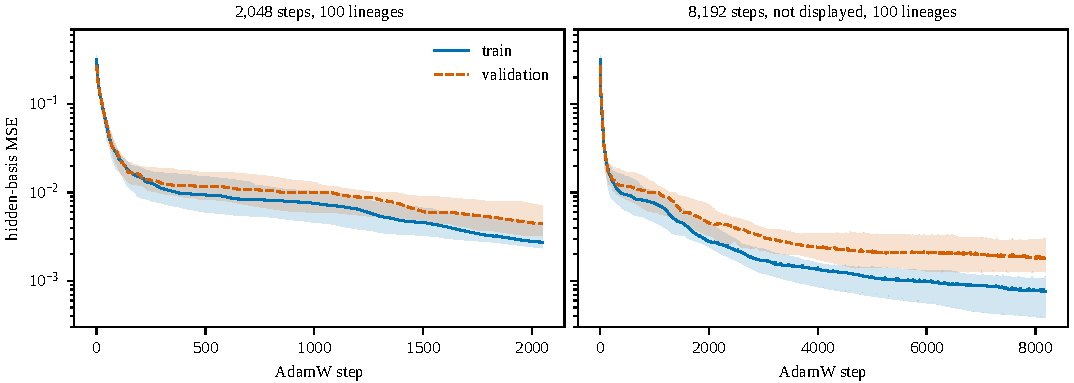
\includegraphics[width=\textwidth]{figures/loss-curves.pdf}
\end{center}

\section{Release score that was not emitted}
\label{app:score}
Equation~(3) of the journal is a gated geometric mean. No artifact in the
journal has a measured value, so this supplement does not print a column
of nulls. Copying a retention number into that scalar would publish a
value the contract refuses to emit. Table~\ref{tab:illustration} applies
the printed formula to invented components
$(0.90, 0.80, 0.85, 0.70, 0.75, 0.95)$. The first
scalar is that formula rounded to two decimals. The all-ones row keeps the
$\epsilon=10^{-6}$ offset, which is why the result is not exactly $100$.
The zero-compactness row uses the same invented components with the
compactness term set to $0$, the value of $\mathrm{clamp}(1 -
\mathrm{bytes}/10240, 0, 1)$ at $10{,}240$ bytes. A failed byte gate is a
different outcome: the implementation returns null and does not emit the
formula. None of these rows was measured.

\begin{table}[t]
\caption{Invented applications of the journal's score formula. Not a measurement.}
\label{tab:illustration}
\centering
\scriptsize
\begin{tabular}{@{}lc@{}}
\toprule
Invented input & Scalar \\
\midrule
Six components above, gates passed & \MfsClassic \\
All six components equal to one & \MfsAllOnes \\
Compactness component set to zero & \MfsZeroCompact \\
Byte gate failed & null \\
\bottomrule
\end{tabular}
\end{table}

\section{Reproducibility}
Regenerate every \texttt{generated/} file, the figure PDFs, and both manuscript PDFs with \texttt{just paper} from the commit that contains these files. That recipe reads the committed validation ledgers, original fit metadata, and compressed numeric replay logs. The replay cost, loss curves, and BeyondArena extracts have file and field mappings in \texttt{generated/original-field-map.json}. Those original metadata snapshots were captured after the historical runs; they do not reconstruct historical custody or replace scored artifacts. Pinned LICENSE extracts are reread when their local store is available. It does not open an official test file. The catalog hash is \CatalogSha. The grouped training split uses seed $\SplitSeed$. The primary displayed DOPE and legacy comparison fits use seed 11 and sample seeds 101, 211, and 307. Later retained panels document additional ARF and Forest-Flow fit seeds and the measured TabSyn and TabDDPM subsets separately. \texttt{python3 research/benchmark/verify\_paper\_numbers.py} exits nonzero when a displayed macro disagrees with those ledgers. Full neural baseline coverage, the pre-specified privacy-attack panel, displayed-DOPE fit-seed variance, and the full ablation grid are named in the prose and omitted from the tables until those runs exist. The journal fidelity table is a separate empirical ledger on the grouped validation split. It is not the pre-specified privacy-attack panel, and it is not differential privacy or HIPAA de-identification.

PMLB is MIT. Every dataset entry in the data lock records SPDX MIT and the note that the source license is MIT (PMLB). CTGAN and TVAE share one pinned LICENSE file: Business Source License 1.1, licensor DataCebo, Inc., licensed work CTGAN. The Gaussian copula uses the pinned Copulas LICENSE: Business Source License 1.1, licensor DataCebo, Inc., licensed work Copulas. TabSyn is Apache License 2.0. TabDDPM is MIT License, Copyright (c) 2022 Akim Kotelnikov. Forest-Diffusion is MIT License, Copyright (c) 2023 Samsung Electronics Co., Ltd. All Rights Reserved. ARF is MIT License, Copyright (c) 2023 Kristin Blesch, Marvin Wright. Chow--Liu and the independent marginals are implementations written for this comparison, under this repository's license: MIT License, Copyright (c) 2026 Dope contributors. The SDV repository LICENSE is not in the pinned snapshot, so that license is not recorded.


Peak RAM in the compute table is resident bytes, shown in mebibytes to
one decimal, and peak VRAM is \texttt{peak\_gpu\_used\_mib}. The hardware
cell names the GPU models recorded on the fit receipts and does not name
a machine. GPU hours sum walls on which the receipt recorded a GPU
process, and each DOPE fit file is counted once. Receipts with no fit
timer are omitted from that table. CPU hours are omitted as well: no
receipt stores a separate CPU timer. The logged replay medians \ReplayMedA\ and \ReplayMedB\ are not
the elapsed time of the scored runs (\CampaignElapsed). Forest-Flow medians use the
\ForestTimeN\ native-grid operation walls. Its bytes are the
$\NForestCb$ selected artifacts. \ForestFitCore\ sums
\texttt{fit\_seconds} and \ForestSampleOp\ sums receipt operations.
Neither sum is that median. Whole-device energy is not job energy.
Gaussian copula, Chow--Liu, and independent-marginal attempts store one
unsplit \texttt{wall\_seconds}. Medians are \GaussAttemptMed,
\ChowAttemptMed, and \IndAttemptMed. Maxima are \GaussAttemptMax,
\ChowAttemptMax, and \IndAttemptMax. BeyondArena medians remain
\BeyondElapseA\ and \BeyondElapseB. Reading the journal threshold
counts from top to bottom, CatBoost is \NThrLowCb, \NThrMidCb,
\NThrHighCb; linear is \NThrLowLin, \NThrMidLin, \NThrHighLin; and the
MLP is \NThrLowMlp, \NThrMidMlp, \NThrHighMlp.

\section{Fit coresets}
\label{app:coreset}
The fit view is not the full PMLB table. Frozen catalog metadata draws each official training and test file by quota stratification on the target distribution and high-variance feature quantile bins, aiming at 1000 training rows and 1000 test rows, with at most 2000 rows in total and at least 101 rows. A source smaller than that quota keeps every row and still reserves a test share of at least 0.2. Of the 100 prepared lineages, 60 were already inside the quota. The other lineages use a hybrid coreset that keeps the observed feature and target range; the bin counts are 1 lineage at 11 bins, and 39 lineages at 50 bins. The generator then groups identical official-training rows and assigns those groups with seed 1729 so that about 80\% of the rows become the fit view and the rest become the validation holdout. Duplicate rows are not split across that cut. On these lineages the fit view has 72 to 800 rows. The bound keeps every lineage on one worker view and leaves the official test sealed. It is not a second draw at scoring time.


\section{Artifact hashes}
\label{app:hashes}
The rows below are SHA-256 of each ledger and round lock the paper reads,
plus the commit and the file hash of the harness that measured the
grouped-validation fidelity ledger. Regenerating the macros does not
rewrite a ledger hash.
{\scriptsize
\begin{longtable}{@{}>{\raggedright\arraybackslash}p{8.6cm}>{\raggedright\arraybackslash}p{8.6cm}@{}}
\toprule
Ledger or lock & SHA-256 \\
\midrule
\endhead
Code commit of the measured harness & \texttt{17f3294d\allowbreak{}139e19f0\allowbreak{}ec831605\allowbreak{}f8750368\allowbreak{}eebc30bb} \\
Harness SHA-256 & \texttt{a952062c\allowbreak{}0f83805f\allowbreak{}6442a440\allowbreak{}a5ae1529\allowbreak{}3a843349\allowbreak{}d423eaa1\allowbreak{}06a9c56a\allowbreak{}20d14c0f} \\
\texttt{research/\allowbreak{}benchmark/\allowbreak{}expanded\_valida\allowbreak{}tion\_metrics.py} & \texttt{a952062c\allowbreak{}0f83805f\allowbreak{}6442a440\allowbreak{}a5ae1529\allowbreak{}3a843349\allowbreak{}d423eaa1\allowbreak{}06a9c56a\allowbreak{}20d14c0f} \\
\texttt{research/\allowbreak{}benchmark/\allowbreak{}methods.lock.jso\allowbreak{}n} & \texttt{899c355c\allowbreak{}b5576971\allowbreak{}0ed369fe\allowbreak{}a6b08258\allowbreak{}9b318588\allowbreak{}60fb7492\allowbreak{}9bf4190d\allowbreak{}e28aca33} \\
\texttt{research/\allowbreak{}benchmark/\allowbreak{}results/\allowbreak{}expanded-validat\allowbreak{}ion-diagnostics.\allowbreak{}json} & \texttt{cd20ac0d\allowbreak{}07a1dcab\allowbreak{}7c5e46db\allowbreak{}195adb46\allowbreak{}3172b517\allowbreak{}4387bb71\allowbreak{}a054b2e5\allowbreak{}f340beeb} \\
\texttt{research/\allowbreak{}benchmark/\allowbreak{}results/\allowbreak{}s3-coreset-proce\allowbreak{}dure.json} & \texttt{73251e43\allowbreak{}cf783868\allowbreak{}74275699\allowbreak{}31bf6127\allowbreak{}f42e9323\allowbreak{}74af3313\allowbreak{}7c57fd8f\allowbreak{}e8544704} \\
\texttt{research/\allowbreak{}benchmark/\allowbreak{}results/\allowbreak{}s3-lineage-recor\allowbreak{}d.json} & \texttt{bbd0852c\allowbreak{}49f59531\allowbreak{}5104261e\allowbreak{}fa4eaa6f\allowbreak{}50db257e\allowbreak{}323b8c00\allowbreak{}2aac6737\allowbreak{}a2dbe7d7} \\
\texttt{research/\allowbreak{}benchmark/\allowbreak{}results/\allowbreak{}density-matched-\allowbreak{}population-valid\allowbreak{}ation.json} & \texttt{5264b88a\allowbreak{}40ad5efb\allowbreak{}21d9b119\allowbreak{}789caeb1\allowbreak{}3e71e911\allowbreak{}a17f1d8b\allowbreak{}57f1d8e8\allowbreak{}ac31732a} \\
\texttt{research/\allowbreak{}benchmark/\allowbreak{}results/\allowbreak{}sdv-matched-popu\allowbreak{}lation-validatio\allowbreak{}n.json} & \texttt{4dc367eb\allowbreak{}78159a03\allowbreak{}86882d23\allowbreak{}ae1f99b0\allowbreak{}aa2cc9f4\allowbreak{}25d1aae4\allowbreak{}99b6f345\allowbreak{}3222a44e} \\
\texttt{research/\allowbreak{}benchmark/\allowbreak{}results/\allowbreak{}s3-matched-fores\allowbreak{}t-confirmation-v\allowbreak{}alidation.json} & \texttt{97a25be9\allowbreak{}02954cad\allowbreak{}16c5b580\allowbreak{}2d0e0ba4\allowbreak{}68dea104\allowbreak{}221efa24\allowbreak{}65434c94\allowbreak{}e6774a1f} \\
\texttt{research/\allowbreak{}benchmark/\allowbreak{}results/\allowbreak{}s3-data.lock.jso\allowbreak{}n} & \texttt{857b6132\allowbreak{}4d0a5b7d\allowbreak{}bbb98e0c\allowbreak{}147fcc79\allowbreak{}c5bb8616\allowbreak{}e7ca61af\allowbreak{}d6785469\allowbreak{}c17f038f} \\
\texttt{research/\allowbreak{}benchmark/\allowbreak{}results/\allowbreak{}arf-native-closu\allowbreak{}re-watch-v1.rece\allowbreak{}ipt.json} & \texttt{7e8eeb1b\allowbreak{}a94ca747\allowbreak{}367e98d5\allowbreak{}a016d2ed\allowbreak{}3ed4c40c\allowbreak{}5a98ca76\allowbreak{}d7a5fe27\allowbreak{}ce9c173c} \\
\texttt{research/\allowbreak{}benchmark/\allowbreak{}results/\allowbreak{}beyondarena-s3-i\allowbreak{}nventory.json} & \texttt{50416676\allowbreak{}4631dbdf\allowbreak{}5e02d116\allowbreak{}334af5cc\allowbreak{}587731fc\allowbreak{}f3efe130\allowbreak{}d62240e6\allowbreak{}dd512d64} \\
\texttt{docs/\allowbreak{}whitepaper/\allowbreak{}generated/\allowbreak{}fit-trace.json} & \texttt{d8c31b9e\allowbreak{}4eb59cb1\allowbreak{}a087cf5d\allowbreak{}cdde4a91\allowbreak{}a73eca00\allowbreak{}f3704fbf\allowbreak{}f647a7da\allowbreak{}6ce65522} \\
\texttt{docs/\allowbreak{}whitepaper/\allowbreak{}generated/\allowbreak{}loss-curves.json} & \texttt{01249154\allowbreak{}97c98e56\allowbreak{}0ef99c1e\allowbreak{}5ecf7ad8\allowbreak{}76f91744\allowbreak{}39ff9c76\allowbreak{}3cf1cf90\allowbreak{}6b4aebe1} \\
\texttt{docs/\allowbreak{}whitepaper/\allowbreak{}generated/\allowbreak{}replay-cost.json} & \texttt{faf77e7c\allowbreak{}e1ed1d22\allowbreak{}127701bf\allowbreak{}68bbfe2f\allowbreak{}8d183f89\allowbreak{}cbd3475d\allowbreak{}d8009488\allowbreak{}8c36f086} \\
\texttt{docs/\allowbreak{}whitepaper/\allowbreak{}generated/\allowbreak{}provenance.json} & \texttt{6880d7d3\allowbreak{}595c0ab9\allowbreak{}ada7396d\allowbreak{}b05513bc\allowbreak{}4be53827\allowbreak{}8e44a510\allowbreak{}334e50e4\allowbreak{}1c7dc7f7} \\
\texttt{docs/\allowbreak{}whitepaper/\allowbreak{}generated/\allowbreak{}beyond-fit.json} & \texttt{a1447f90\allowbreak{}8bc9c518\allowbreak{}76d34559\allowbreak{}7039607c\allowbreak{}734b507b\allowbreak{}f85aa8e0\allowbreak{}8db0639e\allowbreak{}80a1f036} \\
\bottomrule
\end{longtable}
}


\end{document}
